
% Preamble
\documentclass[titlepage]{article}

% Packages
\usepackage{amsmath}
\usepackage{graphicx}
\usepackage{color}
\usepackage[table,xcdraw]{xcolor}
\usepackage{multirow}
\usepackage{float}
\usepackage{booktabs}

\usepackage[margin=2.5cm]{geometry}
\usepackage{hyperref}
\usepackage{varioref}
\usepackage[capitalize]{cleveref}
%\usepackage{nameref}

\usepackage[symbol]{footmisc}


%% Custom commands
\newcommand*\apos{\textsc{\char13}}

% set image file paths
%\graphicspath{ {../../fuzzy/output/mamdani\_bell\_v9/io\_graphs/} }


\title{Fuzzy Systems and Neural Networks}
\author{Jéssica Consciência e Tiago Leite}


\begin{document}
\maketitle
\newpage


\part{Fuzzy System}

%% Texto ainda por melhorar!!
Firstly we started by deciding between which type of fuzzy system
we should implement: Mamdani, Takagi-Sugeno or Tsukamoto.
From the project statement we observe that the output \textit{CLPVariation}
is not any clear function of the input, rulling out Takagi-Sugeno,
also meaning that our output is a \textbf{Fuzzy Set}. If we wish for
our output to be monotonic then the choice would be Tsukomoto, since
we did not want this restriction and decided for starting with a simple
approach then later on adding difficulty when needed.
(Early on we decided to try to make data-driven decisions with an iterative
improving process)

\section{Evaluate Models}

Before we begin defining different system structures with various linguistic variables, terms, and intervals, as well as membership functions, it is essential to establish metrics for evaluating these systems.
By defining appropriate metrics, we can assess their performance objectively and determine which configurations yield the best results.

To achieve this, we implemented the script \texttt{eval\_models.py} (\texttt{fuzzy/eval\_models.py}),
which utilizes a dictionary to compare all model predictions on 10 expert sample data points provided in \newline \texttt{CINTE24-25\_Proj1\_SampleData.csv}.
Initially, the relative error metric, defined as:

\begin{equation*}
    \text{Relative Error} = \frac{|y_{\text{true}} - y_{\text{pred}}|}{y_{\text{true}}}
\end{equation*}

was used for evaluation.
However, this metric exhibited instability when $y_{\text{true}} \to 0$, as was the case for data point 6 in the sample.

%\begin{figure}[htpb]
%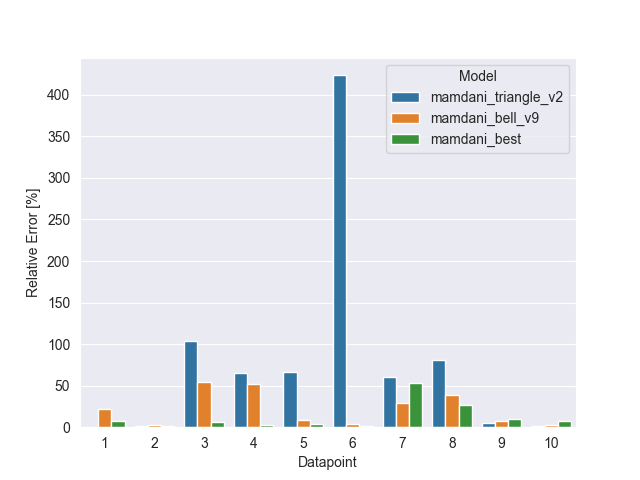
\includegraphics[width=\textwidth]{../images/eval_models/relative_error}
%\end{figure}

To address this instability, we switched to the Mean Squared Error (MSE) metric, defined as:

\begin{equation}
    \text{MSE} = \frac{1}{n} \sum_{i=1}^{n} (y_{\text{true}} - y_{\text{pred}})^2
    \label{eq:mse}
\end{equation}


\section{Architecture}
\subsection{First Iterations}
\label{sec:first_iterations}

In the initial iteration, we selected the variables \textit{ProcessorLoad}, and \textit{MemoryUsage} based on which variables we though were more important.
These variables were chosen as inputs, while \textit{CLP} was designated as the output.
We opted for triangular membership functions, defining four levels for each input variable: (low, medium, high, critical).

We then defined the range of the membership functions associated with each term of the two linguistic variables, \textit{MemoryUsage} and \textit{ProcessorLoad}.
Considering that a device with more than 85\% processor load or memory usage is typically unable to perform its basic tasks,
it became clear that this threshold would correspond to a specific term, labeled as ``critical''.
The ranges for the other membership function terms were distributed between 0 and 1 based on what we deemed appropriate.
We also decided to keep the terms associated with \textit{CLP} straightforward, using only three terms: ``decrease'', ``increase'', and ``maintain''.
The values for the membership functions of these terms were distributed between -1 and 1. The \cref{fig:memory_usage,fig:processor_load,fig:clp} illustrate the membership functions graphs for these variables.

\begin{figure}[H]
    \centering
    \begin{minipage}{0.32\textwidth}
        \centering
        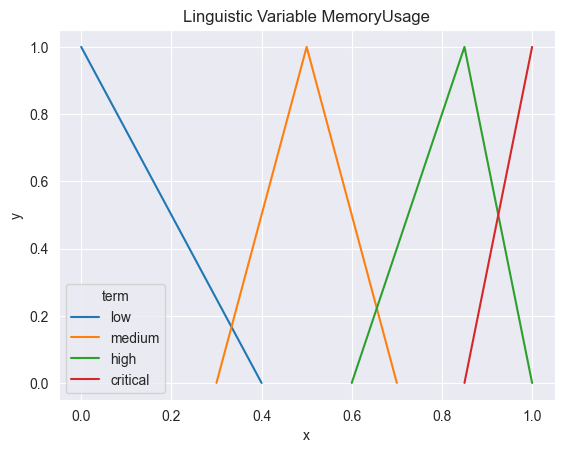
\includegraphics[width=\textwidth]{../images/triangular_MemoryUsage}
        \caption{Memory Usage}
        \label{fig:memory_usage}
    \end{minipage}
    \hfill
    \begin{minipage}{0.32\textwidth}
        \centering
        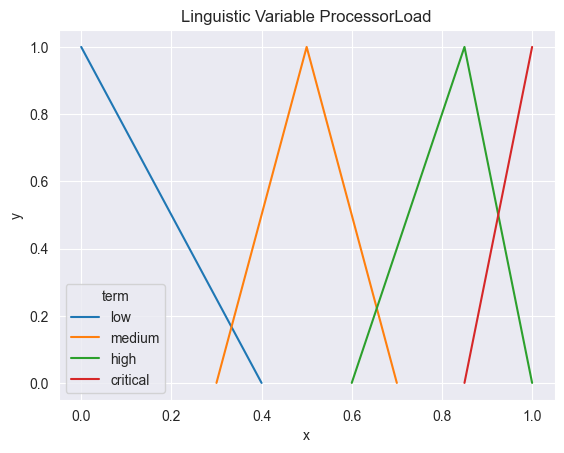
\includegraphics[width=\textwidth]{../images/triangular_ProcessorLoad}
        \caption{Processor Load}
        \label{fig:processor_load}
    \end{minipage}
    \hfill
    \begin{minipage}{0.32\textwidth}
        \centering
        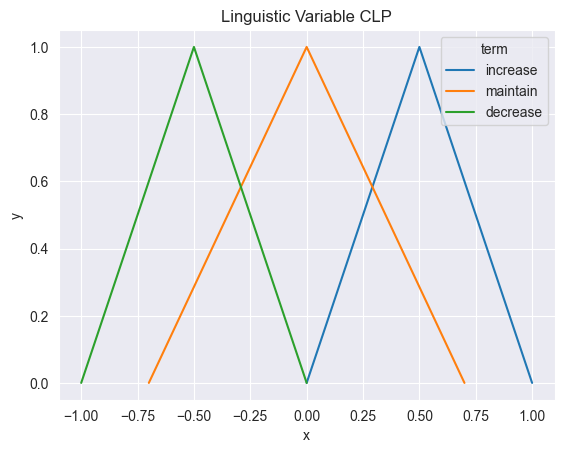
\includegraphics[width=\textwidth]{../images/triangular_CLP}
        \caption{CLP Variation}
        \label{fig:clp}
    \end{minipage}
\end{figure}
\vspace{8mm}

To design the system's rules, we created a truth table, which can be found in~\vref{tab:truthtable}.
The logic behind the table was as follows: when both \textit{MemoryUsage} and \textit{ProcessorLoad} were either ``low'' or ``medium'', the \textit{CLP} would increase.
When one of them reached ``high'', the \textit{CLP} remained unchanged (this decision was made to ensure that the node's processing capacity stayed above average).
Finally, if any of these variables entered a ``critical'' state, the \textit{CLP} had to decrease.


\begin{table}[H]
    \centering
    \begin{tabular}{|
    >{\columncolor[HTML]{9698ED}}c
    >{\columncolor[HTML]{CBCEFB}}c |cccc|}
    \hline
    \multicolumn{2}{|c|}{\cellcolor[HTML]{FFFC9E}}                                         & \multicolumn{4}{c|}{\cellcolor[HTML]{9698ED}ProcessorLoad}                                                                                                                                    \\ \cline{3-6}
    \multicolumn{2}{|c|}{\multirow{-2}{*}{\cellcolor[HTML]{FFFC9E}CPL}}                    & \multicolumn{1}{c|}{\cellcolor[HTML]{CBCEFB}low} & \multicolumn{1}{c|}{\cellcolor[HTML]{CBCEFB}medium} & \multicolumn{1}{c|}{\cellcolor[HTML]{CBCEFB}high} & \cellcolor[HTML]{CBCEFB}critical \\ \hline
    \multicolumn{1}{|c|}{\cellcolor[HTML]{9698ED}}                              & low      & \multicolumn{1}{c|}{increase}                    & \multicolumn{1}{c|}{increase}                       & \multicolumn{1}{c|}{mantain}                      & decrease                         \\ \cline{2-6}
    \multicolumn{1}{|c|}{\cellcolor[HTML]{9698ED}}                              & medium   & \multicolumn{1}{c|}{increase}                    & \multicolumn{1}{c|}{increase}                       & \multicolumn{1}{c|}{maintain}                     & decrease                         \\ \cline{2-6}
    \multicolumn{1}{|c|}{\cellcolor[HTML]{9698ED}}                              & high     & \multicolumn{1}{c|}{maintain}                    & \multicolumn{1}{c|}{maintain}                       & \multicolumn{1}{c|}{maintain}                     & Decrease                         \\ \cline{2-6}
    \multicolumn{1}{|c|}{\multirow{-4}{*}{\cellcolor[HTML]{9698ED}MemoryUsage}} & critical & \multicolumn{1}{c|}{Decrease}                    & \multicolumn{1}{c|}{Decrease}                       & \multicolumn{1}{c|}{Decrease}                     & Decrease                         \\ \hline
    \end{tabular}
    \caption{Truth table}
    \label{tab:truthtable}
\end{table}

\vspace{8mm}

To visualize the system's output, we generated 50 data points for \textit{MemoryUsage} and \textit{ProcessorLoad} ranging between 0 and 1.
We then created an interactive 3D plot that showed the evolution of \textit{CLP} based on these two values, this can be seen in \cref{fig:3d_triangular}.
Upon reviewing the graph, we noticed that the variables \textit{ProcessorLoad} and \textit{MemoryUsage} exhibited very similar behavior because intuitively, when designing the system, we had structured the membership functions for each term in the same way for both variables, and the truth table was also symmetric.
This indicates that the system should react in the same way to both variables and they could, in fact, be merged into a single variable without losing the system's effectiveness.
By combining these two variables, we simplify the model while still accurately representing the system's behavior, as both variables seem to influence the \textit{CLP} in a nearly identical manner.


\begin{figure}[H]
    \centering
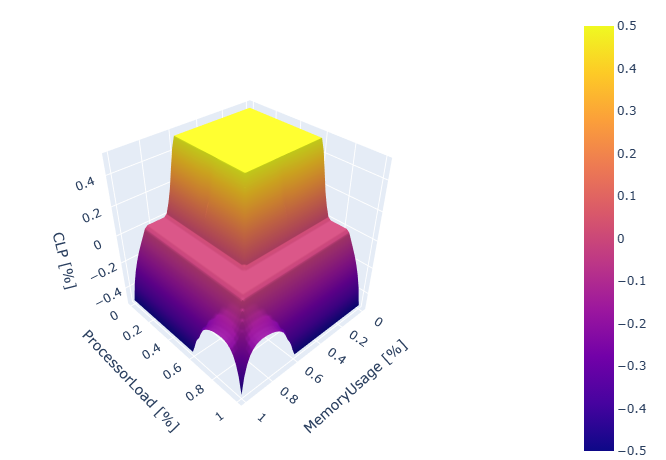
\includegraphics[scale = 0.7]{../images/3d_triangular}
\caption{Fuzzy CLP Inference}
\label{fig:3d_triangular}
\end{figure}

%\vspace{10mm}

From the graph we also noticed that the \textit{CLP} only varies between -0.5 and 0.5, which is not the desired range; we aim for it to vary between -1 and 1.
This limitation is due to the configurations of the membership functions for the terms ``increase'' and ``decrease'' of the \textit{CLP}.
Additionally, two constant plateau regions are visible where the \textit{CLP} remains unchanged: when \textit{MemoryUsage} and \textit{ProcessorLoad} are between 0 and 0.6, and when they are between 0.7 and 0.85, which does not make sense in our context.
Finally, in the area of the graph where \textit{CLP} is less than -0.2 and \textit{MemoryUsage}/\textit{ProcessorLoad} is greater than 0.6, there is a ``hump'' with no \textit{CLP} values, which is undesirable.
\newline

Subsequently, we explored the effect of switching the membership functions to a Gaussian distribution because they provide a smoother transition between membership grades.
To make a direct comparison with the system we previously developed using triangular membership functions, we retained the same linguistic variables, the same terms for these variables, and the same rules as presented in~\cref{tab:truthtable}.

\begin{figure}[H]
    \centering
    \begin{minipage}{0.45\textwidth}
        \centering
        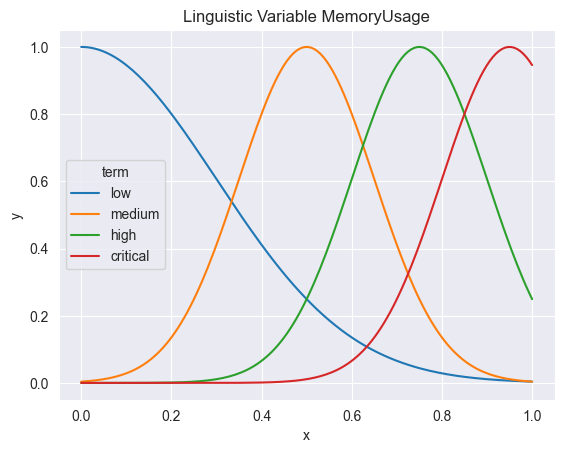
\includegraphics[width=\textwidth]{../images/guassian_MemoryUsage}
        \caption{Memory Usage MF}
        \label{fig:memory_usage_gaussian}
    \end{minipage}
    \hfill
    \begin{minipage}{0.45\textwidth}
        \centering
        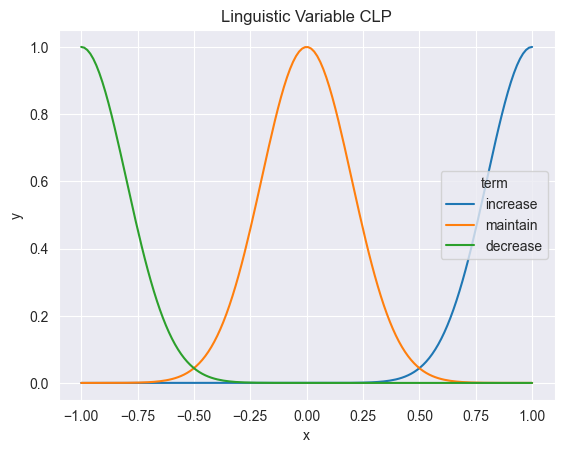
\includegraphics[width=\textwidth]{../images/guassian_CLP}
        \caption{CLP Variation MF}
        \label{fig:clp_gaussian}
    \end{minipage}
\end{figure}

\vspace{10mm}

The resulting 3D graph showing the variation of the \textit{CLP} with \textit{MemoryUsage} and \textit{ProcessorLoad} can be seen in Figure~\ref{fig:3d_gaussian}

\begin{figure}[H]
    \centering
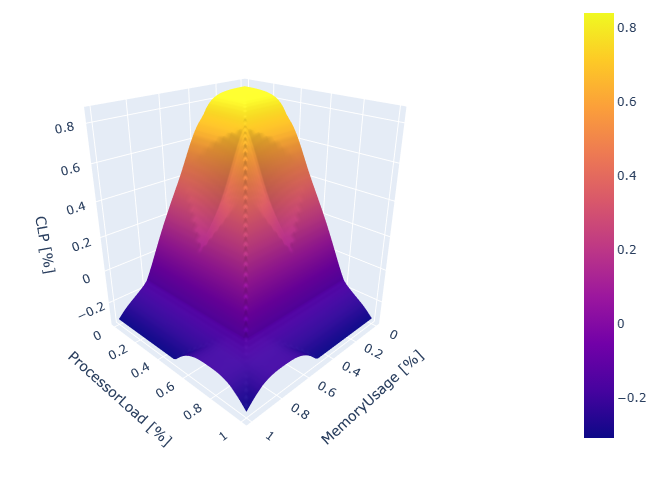
\includegraphics[scale = 0.7]{../images/3d_guassian}
\caption{Fuzzy CLP Inference using Guassians as MF}
\label{fig:3d_gaussian}
\end{figure}

\vspace{10mm}


This time, the system achieved higher positive \textit{CLP} values, but it worsened on the negative \textit{CLP} values, only going down to -0.2.
To achieve better results, we decided to add more terms to the linguistic variables, merge \textit{MemoryUsage} with \textit{ProcessorLoad} into a single variable, and experiment with different membership functions. By increasing the number of terms, we aim to capture more detailed nuances in the system's behavior, improving its responsiveness to variations in input. Additionally, merging the two load-related variables simplifies the model without losing critical information. The next sections will address these adjustments in detail, explaining the rationale behind these changes and the impact they have on the system's performance.


\subsection{Generalized Bell}
\subsubsection{Bell v9}
\label{sec:bell_v9}
We decided to experiment using a more generic Membership function, so we
extended simpful's Base Membership Function class and created Bell\_MF [in fuzzy/models/bell\_mf.py].
The Generalized Bell has parameters $a$, $b$ and $c$ that are responsible for the slope\footnote[1]{The slope of the function is influenced by both parameters $a$ and $b$, where $slope = \frac{a}{2b}$}, width, and center of the function, respectively.
\newline
\newline
First, we decided to combine the variables \textit{ProcessorLoad} and \textit{MemoryUsage} into a single variable: \textit{SystemLoad}, which is defined as the maximum value between these two variables. We chose the maximum value because it allows us to capture the most critical resource constraint affecting system performance. By focusing on the highest load, the system can respond to the most demanding condition, ensuring that performance is not compromised under heavy usage. Then we added two more terms to the CLP variable (``increase\_significantly'' and ``decrease\_significantly'') to capture additional complexity in the model.


\newline
After extensive manual iteration the best performing model (\textbf{bell\_v9}) has the following linguistic variables and terms illustrated in the following~\cref{fig:bellv9_system_load,fig:bellv9_latency,fig:bellv9_clp}.
\begin{figure}[H]
    \centering
    \begin{minipage}{0.32\textwidth}
        \centering
        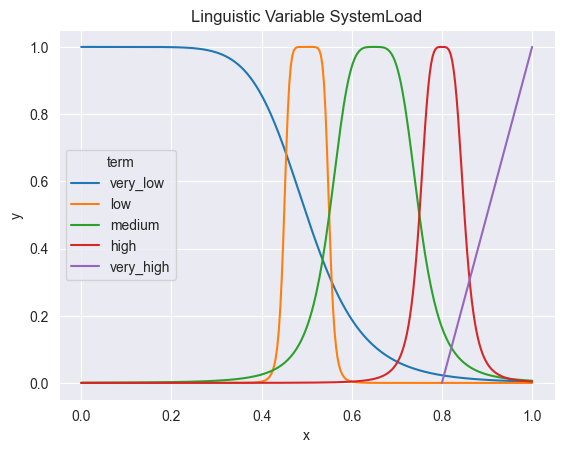
\includegraphics[width=\textwidth]{../images/bell_v9/SystemLoad}
        \caption{SystemLoad}
        \label{fig:bellv9_system_load}
    \end{minipage}
    \hfill
    \begin{minipage}{0.32\textwidth}
        \centering
        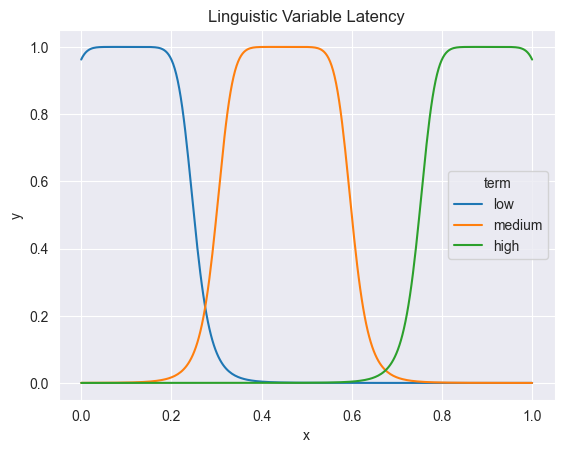
\includegraphics[width=\textwidth]{../images/bell_v9/Latency}
        \caption{Latency}
        \label{fig:bellv9_latency}
    \end{minipage}
    \hfill
    \begin{minipage}{0.32\textwidth}
        \centering
        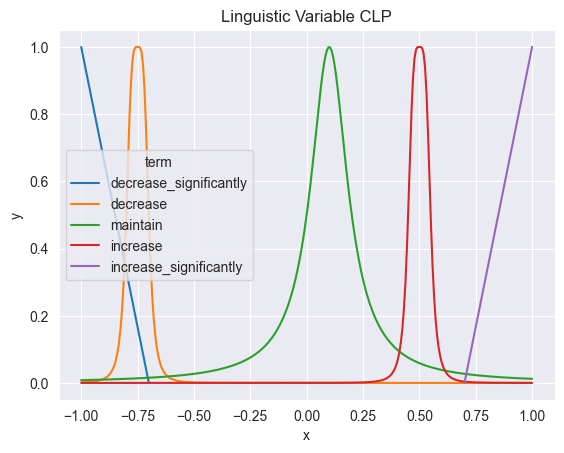
\includegraphics[width=\textwidth]{../images/bell_v9/CLP}
        \caption{CLP Variation}
        \label{fig:bellv9_clp}
    \end{minipage}
    %\caption{Fuzzy Sets Bell v9}
    %\label{fig:fuzzy_sets_bellv9}
\end{figure}

This model obtained an \emph{MSE}$=0.0447$ on the expert dataset.

\subsubsection{Bell Hypertuned}
Using the \texttt{bell\_v9} model obtained in section \cref{sec:bell_v9} as a base, including its linguistic variables and rule base, we conducted a thorough hyperparameter tuning of the parameters $a$, $b$, and $c$ of the membership functions.
This procedure is explained in more detail in the section~\nameref{sec:hyper_tuning}.

After 3 hours of hyperparameter tuning, the resulting \texttt{bell\_hyper} model, comprising a total of 6228 trials, achieved a final total MSE of $0.00749$ (using the 10 expert data points).  
This corresponds to a six-fold improvement over the manually obtained \emph{MSE} of $0.04473$ for the \texttt{bell\_v9}.

The best hyperparameters from this tuning process were saved as \texttt{hparams\_007.json}.
The resulting linguistic variables are shown in the following~\cref{fig:bell_hyper_system_load,fig:bell_hyper_latency,fig:bell_hyper_clp}.

\begin{figure}[H]
    \centering
    \begin{minipage}{0.32\textwidth}
        \centering
        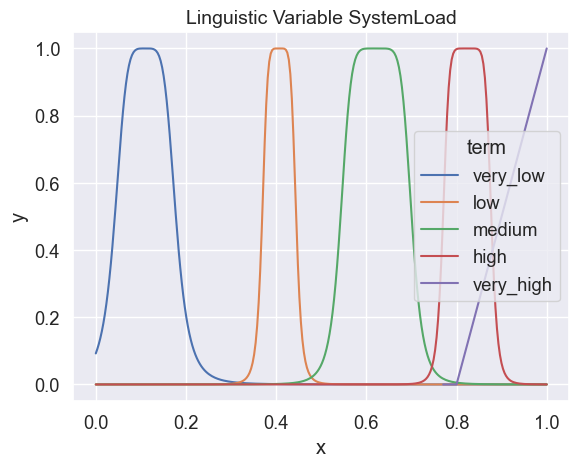
\includegraphics[width=\textwidth]{../../fuzzy/output/mamdani_bell_hyper/io_graphs/SystemLoad}
        \caption{SystemLoad}
        \label{fig:bell_hyper_system_load}
    \end{minipage}
    \hfill
    \begin{minipage}{0.32\textwidth}
        \centering
        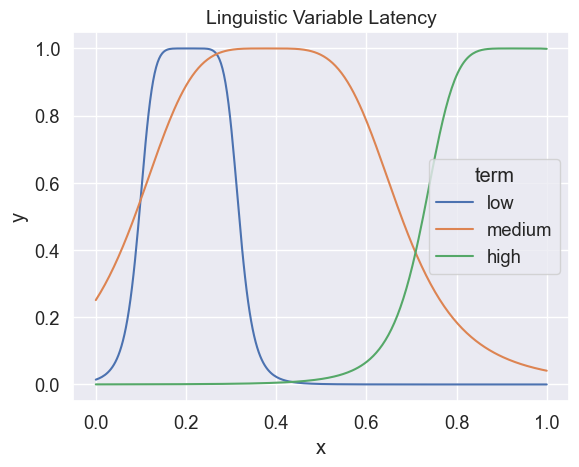
\includegraphics[width=\textwidth]{../../fuzzy/output/mamdani_bell_hyper/io_graphs/Latency}
        \caption{Latency}
        \label{fig:bell_hyper_latency}
    \end{minipage}
    \hfill
    \begin{minipage}{0.32\textwidth}
        \centering
        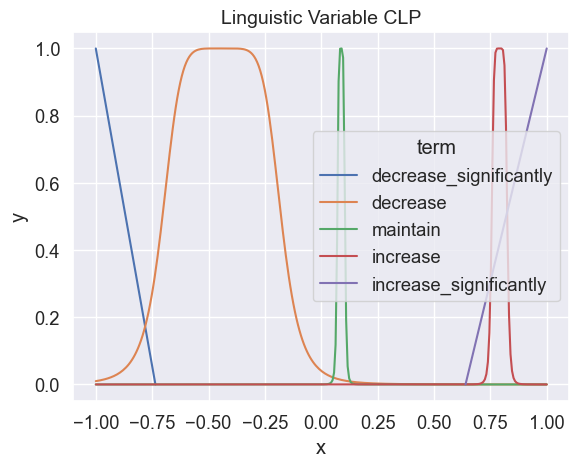
\includegraphics[width=\textwidth]{../../fuzzy/output/mamdani_bell_hyper/io_graphs/CLP}
        \caption{CLP Variation}
        \label{fig:bell_hyper_clp}
    \end{minipage}
    %\label{fig:fuzzy_sets_bell_hyper}
\end{figure}

For the linguistic variable \emph{Latency} (\cref{fig:bell_hyper_latency}), we observe that for values close to $0$, it is considered \emph{medium}, then \emph{low}, and back to \emph{medium} again at around $x = 0.38$, which does not make sense.
Additionally, for the linguistic variable \emph{CLP} (\cref{fig:bell_hyper_clp}), we observe that between \emph{maintain} and \emph{increase}, there is a large section where the membership value is $0$, which is undesirable for a real Fuzzy System.
These problems are likely the result of overfitting and may also be due to the low number of points in the expert dataset.


\subsection{Triangle Version Improved (triangle\_v4)}


Since we believe the model from the previous section is overfitting and some membership functions do not seem logical, we decided to start again from the system with triangular membership functions presented in Section~\ref{sec:first_iterations}, and we iteratively built a new system.



We decided to assign the same terms we had initially used for the variables \textit{MemoryUsage}/\textit{ProcessorLoad} to the new variable \textit{SystemLoad}, namely: ``low'', ``medium'',``high'', and ``critical.'' As for the output variable, \textit{CLP}, we decided to add two new terms: ``increase\_significantly'' and ``decrease\_significantly''.

The values a, b, and c that define the triangles of the membership functions were chosen through an iterative process, where we adjusted some of the boundaries (both for the terms related to \textit{SystemLoad} and for the terms of \textit{CLP}) and observed the resulting defuzzified \textit{CLP}.
We then evaluated whether the results made sense, given the system's requirements. For example, if the \textit{SystemLoad} input was 0.9, it would not make sense for the resulting \textit{CLP} to be 0.7. Based on this logic, we continued adjusting the limits of the membership functions iteratively.

Later, when we gained access to expert data, this process became easier, as we had a ground truth to reference.
This allowed us to test our system and evaluate it using more quantitative metrics.
However, this process was quite exhaustive, as improving the error for one set of data sometimes worsened the results for others.
Ultimately, we arrived at the following membership functions for each term of each variable.

\begin{figure}[H]
    \centering
    \begin{minipage}{0.45\textwidth}
        \centering
        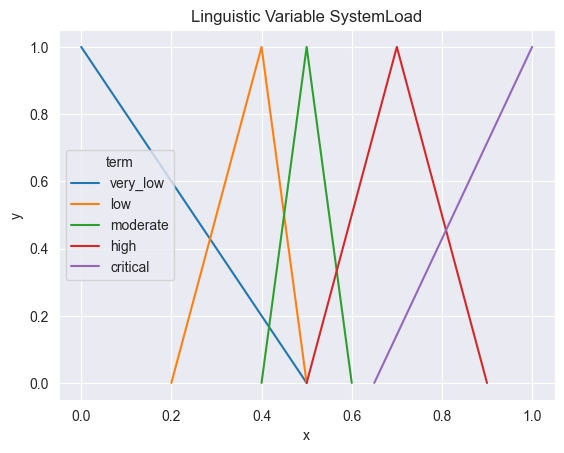
\includegraphics[width=\textwidth]{../images/triangular_v4_SystemLoad}
        \caption{SystemLoad MF`s}
        \label{fig:systemload_triangular_v4}
    \end{minipage}
    \hfill
    \begin{minipage}{0.45\textwidth}
        \centering
        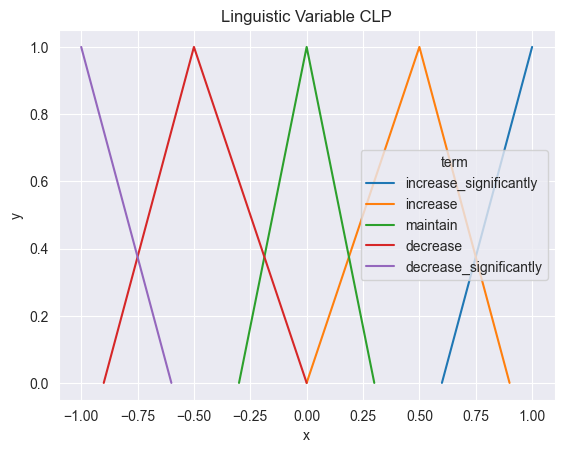
\includegraphics[width=\textwidth]{../images/triangular_v4_CLP}
        \caption{CLP Variation MF`s}
        \label{fig:clp_triangular_v4}
    \end{minipage}
\end{figure}

\vspace{5mm}


Initially, the system only considered a single variable, \textit{SystemLoad}.
However, with the data provided to us, we realized that this variable alone was not sufficient to capture all the nuances of the real system.
There were additional aspects we needed to address using other variables.
As a result, we decided to introduce another linguistic variable: \textit{Latency}.

We defined three terms for the linguistic variable \textit{Latency}: ``low'', ``moderate'', and ``high''.
Similar to the approach used for \textit{SystemLoad}, the membership functions were established iteratively, using a trial-and-error process based on what we considered reasonable.
The membership functions for \textit{Latency} are illustrated in \cref{fig:latency_triangular_v4}.

\begin{figure}[H]
    \centering
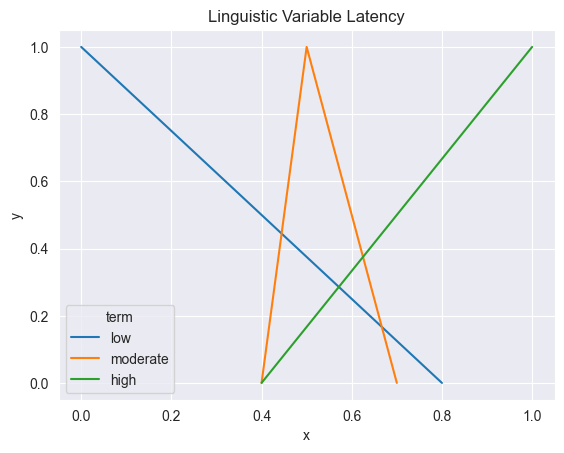
\includegraphics[scale = 0.6]{../images/triangular_v4_latency}
\caption{Latency MF}
\label{fig:latency_triangular_v4}
\end{figure}

%\vspace{5mm}


The logic we followed when adding rules was based on the following statement: ``high latency means that it’s better to process data locally'', we determined that in cases where \textit{SystemLoad} is high, the \textit{CLP} could either be maintained at an increasing value or reduced to offload processing to the cloud.
However, this decision heavily depends on latency: if latency is low, we can process the data in the cloud (which implies slightly lowering the \textit{CLP}), but if latency is high, it is preferable to continue processing locally on the node since the communication channel is experiencing significant delays.


In the graph shown in \cref{fig:3d_latency_triangular_v4}, the variation of \textit{CLP} with \textit{SystemLoad} and \textit{Latency} is represented.
We can observe that when \textit{SystemLoad} is between 0.6 and 0.75, the \textit{CLP} varies with \textit{Latency}: with low latency, the \textit{CLP} decreases, whereas with high latency, the \textit{CLP} increases.

\begin{figure}[H]
    \centering
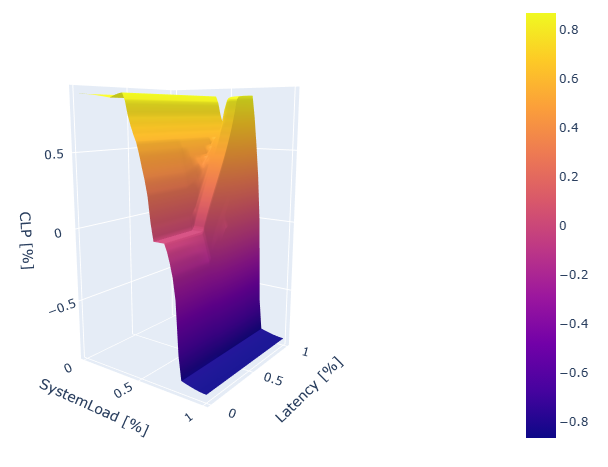
\includegraphics[scale = 0.6]{../images/3d_triangular_v4_latency}
\caption{3D plot of CLP variation with Latency and SystemLoad}
\label{fig:3d_latency_triangular_v4}
\end{figure}

%\vspace{8mm}


Finally, we introduced another variable: \textit{OutBandwidth}, as moving data to the cloud (when we reduce computation) is limited by the available bandwidth.
Therefore, when the \textit{SystemLoad} was critical and it was necessary to reduce the \textit{CLP} to negative values, the amount by which the \textit{CLP} would decrease would depend on the available bandwidth: when bandwidth was high, the \textit{CLP} would decrease significantly (``decreased\_significantly''), and when bandwidth was medium or low, the \textit{CLP} would only decrease slightly (``decrease'').
In Figure~\cref{fig:bandwidth_triangular_v4}, the terms and membership functions of the variable \textit{OutBandwidth} are represented.

\begin{figure}[H]
    \centering
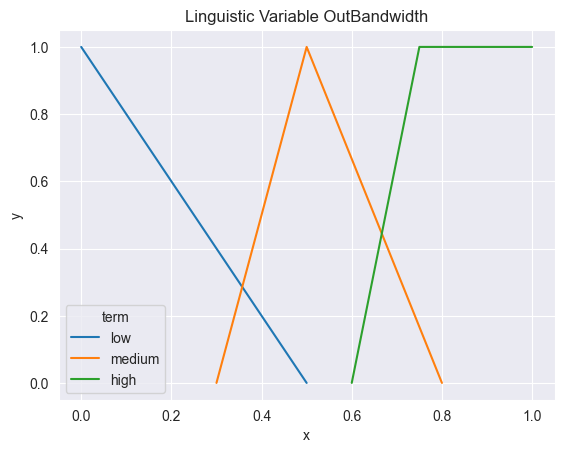
\includegraphics[scale = 0.6]{../images/triangular_v4_OutBandwidth}
\caption{OutBandwidth MF}
\label{fig:bandwidth_triangular_v4}
\end{figure}


We evaluated the system using the 10 data points provided, this model (\texttt{triangle\_v4}) achieved the lowest Mean Squared Error (MSE) of 0.00735.
In Figure~\ref{fig:MSE_triangle_v4.png}, a graph illustrates the contribution of each data point to the overall MSE. Notably, points 4, 6, 7, and 8 have the most significant contributions to the error; however, they remain below 0.0016.
The system behaves as expected, increasing the \textit{CLP} when necessary and decreasing it at appropriate times, while taking into account the constraints of edge computing and the requirements for offloading processing to the cloud.

\begin{figure}[H]
    \centering
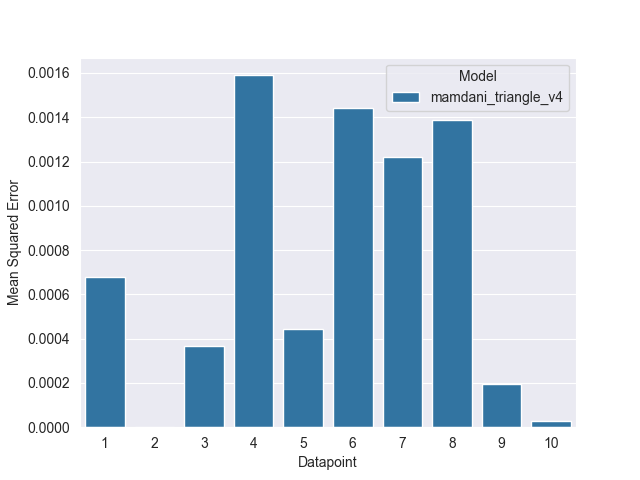
\includegraphics[scale = 0.5]{../images/MSE_triangle_v4}
\caption{MSE of each point of experts dataset}
\label{fig:MSE_triangle_v4.png}
\end{figure}

%During the experimentation phase with different membership functions,the need for visualization became apparent.
%To facilitate this, we developed a helper script [fuzzy/visualization/fuzzy\_system\_to\_dataframe] that converts the
%FuzzySystem Python object into a dynamic dataframe, enabling easy plotting and analysis of the membership functions.


\section{Hyperparameter Tuning}
\label{sec:hyper_tuning}

%Since we had manually iterated until a good model was reached, scoring 0.0447 in total MSE on the 10 sample data points, we considered the linguistic variables and rule base as fixed.
We found ourselves tirelessly fine-tuning the membership functions, such as the center, slope, and width in the case of the bell membership function.
To automate this process, we took the following steps:

\begin{itemize}
    \item Create a \texttt{FuzzySystem} from a set of hyperparameters [\texttt{fuzzy/models/mamdani\_hparams.py}].
    \item Define an objective function to minimize/maximize.
          In our case, we used the total MSE of the 10 sample data points as the objective value to be minimized.
    \item Sample several hyperparameter trials and find the best.
          This was done with the help of the Python framework \texttt{optuna}, which uses Bayesian Optimization to find optimal hyperparameters.
\end{itemize}

A simpler approach would have been to use \texttt{RandomSearch} or \texttt{GridSearch} (possibly using \texttt{scikit-learn}).
However, we chose to leverage \texttt{optuna}\apos s search algorithm, Tree Parzen Estimation (TPE).
In a nutshell, TPE builds an internal model that makes ``educated'' guesses about which hyperparameters to test and continuously updates that model.
The search is then performed in a tree-like manner, and \texttt{optuna} can handle both continuous and categorical data.

After 3 hours of hyperparameter tuning, the \texttt{mamdani\_bell\_v9} model, comprising a total of 6228 trials, achieved a final total MSE of $0.00749$.
This corresponds to a six-fold improvement over the manually obtained $MSE$ of $0.04473$.
The best hyperparameters from this tuning process were saved as \texttt{hparams\_007.json}.


\section{Conclusion}

Now we present a more precise examination of the best models: \texttt{bellv9}, \texttt{bell\_hyper}, and \texttt{triangle\_v4}.
What follows is the evaluation using the MSE metric for the 10 sample data points, shown in the \vref{fig:mse_3best}.

\begin{figure}[H]
\centering
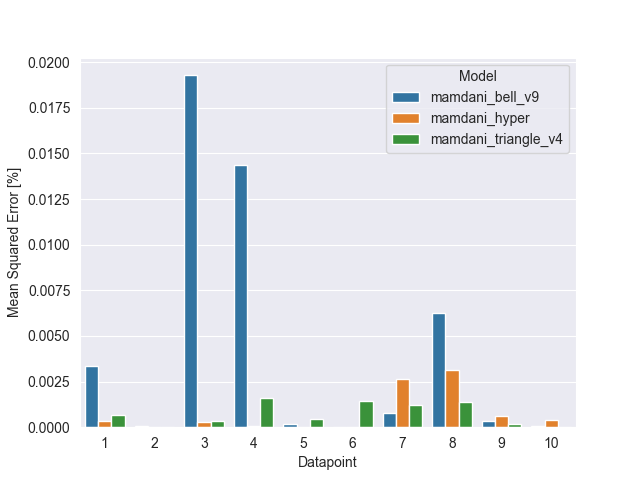
\includegraphics[scale=0.4]{../images/eval_models/mse_3best}
\caption{MSE of the top 3 performing models (\texttt{bellv9}, \texttt{bell\_hyper}, and \texttt{triangle\_v4})}
\label{fig:mse_3best}
\end{figure}

In the next \cref{fig:mse_2best}, we compare only the best two models.

\begin{figure}[H]
\centering
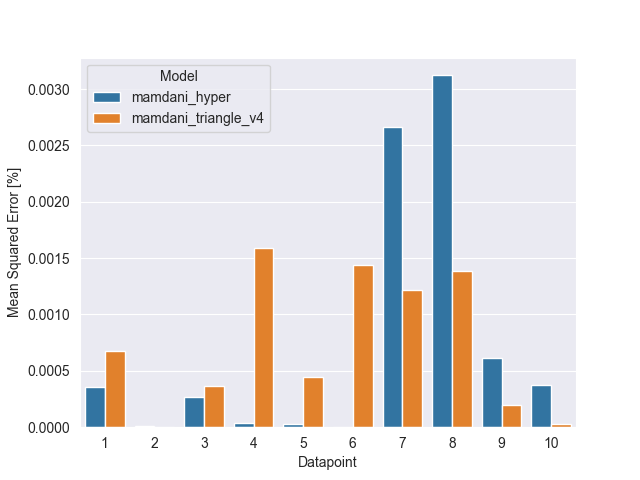
\includegraphics[scale=0.4]{../images/eval_models/mse_2best}
\caption{MSE of the top 2 performing models (\texttt{bell\_hyper}, and \texttt{triangle\_v4})}
\label{fig:mse_2best}
\end{figure}

We can observe that they appear to score similarly, with the total score of \texttt{triangle\_v4} being slightly better than \texttt{bell\_hyper} ($0.735 < 0.749$).
However, the membership functions are drastically different (see FIGURE for \texttt{bell\_hyper} and \cref{fig:systemload_triangular_v4,fig:clp_triangular_v4,fig:latency_triangular_v4} for \texttt{triangle\_v4}).
The membership functions of \texttt{triangle\_v4} are much more understandable and interpretable, whereas those of \texttt{bell\_hyper} seem to be a result of overfitting.
\\
This evaluation process was instrumental in improving our models and identifying potential problem areas.
For instance, the model consistently underestimated the CLP for data points 3 and 4, this is shown in the table below.

\begin{table}[H]
    \centering
    \caption{Sample data points 3 and 4}
    \label{tab:datapoints_3_4}
    \begin{tabular}{lrrrrr}
        \toprule
        & MemoryUsage & ProcessorLoad & Latency & mamdani\_bell\_v2 & CLPVariation \\
        \midrule
        3 & 0.68        & 0.60          & 0.80    & 0.30              & 0.73         \\
        4 & 0.50        & 0.50          & 0.50    & 0.66              & 0.50         \\
        \bottomrule
    \end{tabular}
\end{table}



These observations suggested, in our view, that the model should account for high latency as a factor contributing to a lower \emph{CLP}.
This iterative process led to the development of models like \texttt{mamdani\_triangle\_v2} and \texttt{mamdani\_bell\_v9}.\\
Many more iterations were tested but not preserved.
Some of the deprecated models can still be found in the \texttt{fuzzy/models/deprecated} folder, along with their outputs in \texttt{fuzzy/output/deprecated}.

The best model, \texttt{mamdani\_best}, emerged as the result of extensive hyperparameter tuning, which is discussed in detail in the~\nameref{sec:hyper_tuning} section.




\part{Neural Networks}

\section{Architecture}

To build the neural network, we decided to use a simple architecture: 3 layers (one input layer, one hidden layer and one output layer), 12 input nodes, 32 nodes in the hidden layer, and 1 output node.
Since the output should be in the range \([-1, 1]\), we chose the \emph{Tanh} activation function, which produces values within this range.
For the optimizer, we used Adam with a learning rate of $1 \times 10^{-3}$, leaving the rest of the parameters at their default values: $\epsilon = 1 \times 10^{-8}$, $\beta = (0.9, 0.999)$, and \texttt{weight\_decay} = 0.
For the loss function, we chose MSE, allowing us to directly compare the results with those of the Fuzzy System.

We implemented the neural network using the PyTorch framework alongside \newline \texttt{pytorch\_lightning}.
This made it easy to integrate TensorBoard for logging and visualization, apply Early Stopping to prevent unnecessary computation, and enable Model Checkpointing to save the best-performing model.
This code can be found in the \texttt{nn/models/simple\_lightning.py} file.

\section{Training Data}

To create the training data for the neural network, we began by generating synthetic data for the $12$ input features.
This was done by sampling $100.000$ random uniformly distributed values for each feature.
Next, the Fuzzy System was used to predict the CLPVariation, utilizing the best-performing Fuzzy System located in \texttt{fuzzy/models/mamdani\_best.py}.
The results were then stored in a CSV file inside the \texttt{gen\_input} folder.
This code can be found in the \texttt{fuzzy/generate\_data.py} file.
The decision to use random uniform data, as opposed to, for example, a Gaussian distribution, was made to ensure a \textbf{balanced} dataset for training the neural network.
The choice of the number of training data samples was also carefully considered.
We followed the rule of thumb that ``a model will often need ten times more data than it has degrees of freedom'', where a degree of freedom refers to model parameters or input features.
Our model has 449 trainable parameters and 12 input features, which means our training data should consist of more than $4610$ samples.
We decided to generate a number of samples equal to an order of magnitude above 4610 rounded up, which results in 100,000 samples.

\section{Classification}

To use the neural network as a classifier, we first defined the ground truth intervals as \([-1, 0.3[\) for \emph{Decrease}, \([0.3, 0.5[\) for \emph{Maintain}, and \([0.5, 1]\) for \emph{Increase}, based on the CLP linguistic variable intervals as shown in the figure below.

Using these intervals, we labeled the training, validation, and test data for the neural network.
Next, we labeled the data again using the same intervals but with the results predicted by the neural network.
The confusion matrix heatmap showing these results is \cref{fig:confusion_matrix_heatmap}.

\begin{figure}[H]
\centering
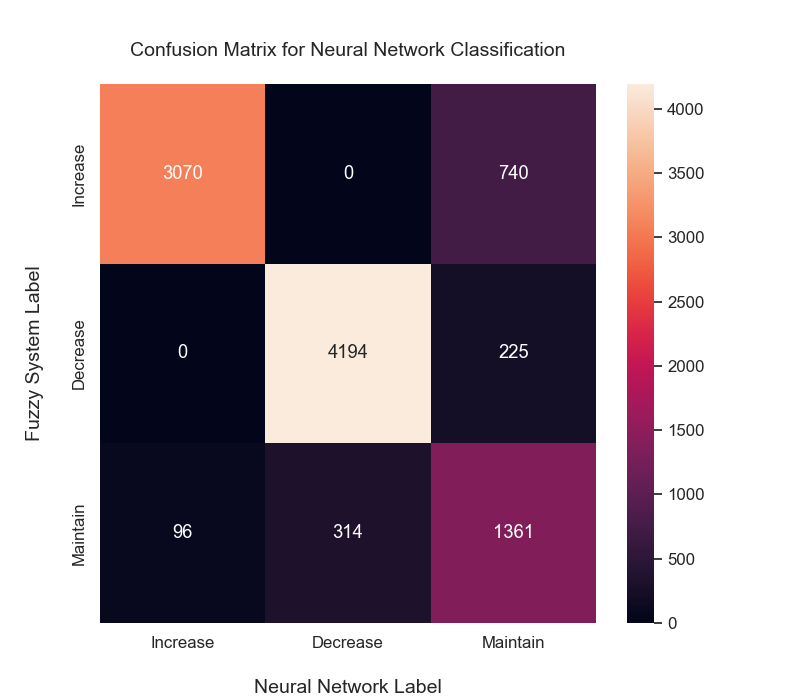
\includegraphics[scale=0.4]{../images/classification/confusion_heatmap}
\caption{Confusion Matrix Heatmap}
\label{fig:confusion_matrix_heatmap}
\end{figure}

To gain a better understanding of the neural networks performance, we calculated the Precision, Recall, and F1-score, which are shown in the table below.

\begin{table}[H]
    \centering
    \caption{}
    \label{tab:classification_scores}
    
\begin{tabular}{rrrl}
\toprule
precision & recall & f1-score & label \\
\midrule
0.96 & 0.97 & 0.96 & Decrease \\
0.97 & 0.89 & 0.93 & Maintain \\
0.19 & 0.36 & 0.25 & Increase \\
\bottomrule
\end{tabular}

\end{table}


\end{document}
